\documentclass[12pt,oneside]{exam}

% This package simply sets the margins to be 1 inch.
\usepackage[margin=1in]{geometry}

% These packages include nice commands from AMS-LaTeX
\usepackage{amssymb,amsmath,amsthm,amsfonts,latexsym,verbatim,xspace,setspace, graphicx}
\usepackage{subfigure}

% Make the space between lines slightly more
% generous than normal single spacing, but compensate
% so that the spacing between rows of matrices still
% looks normal.  Note that 1.1=1/.9090909...
\renewcommand{\baselinestretch}{1.1}
\renewcommand{\arraystretch}{.91}

% Define an environment for exercises.
\newenvironment{exercise}[1]{\vspace{.1in}\noindent\textbf{Exercise #1 \hspace{.05em}}}{}
\newenvironment{newsolution}{\vspace{.1in}\noindent\textbf{Solution \hspace{.05em}}}{}

% define shortcut commands for commonly used symbols
\newcommand{\R}{\mathbb{R}}
\newcommand{\C}{\mathbb{C}}
\newcommand{\Z}{\mathbb{Z}}
\newcommand{\Q}{\mathbb{Q}}
\newcommand{\N}{\mathbb{N}}
\newcommand{\calP}{\mathcal{P}}

\DeclareMathOperator{\vsspan}{span}

\title{Math 203 - Summer II 2018: Solutions to homework 3}

%%%%%%%%%%%%%%%%%%%%%%%%%%%%%%%%%%%%%%%%%%

\begin{document}

\begin{flushright}
\sc MAT 203 - Lecture 1\\
August 9, 2018.
\end{flushright}
\bigskip

\begin{center}
\textsf{Homework 3: solutions to selected problems} 
\end{center}

\begin{exercise}{1}
In class, we characterized the gradient of a differentiable function $f$ at a point $p$ geometrically as a vector which points in the directtion of maximum increase of the function. We also characterized it analytically as the vector encoding the best linear approximation of the function, 
\begin{equation*}
f(p)=f(p_0)+\nabla f(p_0) \cdot (p-p_0) + O(||p-p_0||), 
\end{equation*}
where $O(||p-p_0||)$ simbolizes an error term whose magnitude is small relative to that of $||p-p_0||$ ( a notion which can be made precise with multivariable limits). With this at hand, we saw in class that (for functions with continuous partial derivatives) the gradient can be expressed in a simple way using partial derivatives:
\begin{equation}\label{gradient}
\nabla f(p_0) = \left[\frac{\partial f}{\partial x} (p_0)\right]i + \left[\frac{\partial f}{\partial y} (p_0)\right] j  + \left[\frac{\partial f}{\partial z} (p_0)\right] k,
\end{equation}
the partial derivative relative to $z$ being absent when $f$ is a function of two variables only. 

In this exercise will see how the gradient relates to the notion of directional derivatives discussed earlier in the course. In the rest of this problem, $f$ denotes the function $f(x,y,z)=4x^2+3yz+2z$. 

\begin{itemize}
\item[(a)] Compute its gradient vector at a point $(x,y,z)$ using the formula given above. 
\item[(b)] Use the definition of directional derivative (as a directed limit) to compute the directional derivative of $f$ at $(0,0,0)$ in the direction 
\begin{equation*}
v=\left(\frac{1}{\sqrt 3}, \frac{1}{\sqrt 3},\frac{1}{\sqrt 3}\right).
\end{equation*}
\item[(c)] Compute the dot product between the gradient you found in part (a), at the point $(0,0,0)$, and the vector $v$ from part $b$. 
\end{itemize}

Your results from parts (b) and (c) should have been the same. In fact, this is the takeaway from this problem: \textit{for functions with continous partial derivatives, the gradient vector field can be used to compute directional derivatives}. The directional derivative of $f$ in the direction of $v$ at a point is given by the dot product between its gradient vector at that point and the direction $v$. 
\end{exercise}

\begin{newsolution}
\begin{itemize}
\item[(a)] 
\begin{equation*}
\nabla_{f} (x,y,z)=8x i + 3zj + (3y+2)k
\end{equation*}
\item[(b)] 
\begin{align*}
\frac{\partial f}{\partial v} (0,0,0) & = \lim_{t \to 0} \frac{f\left((0,0,0)+t\left(\frac{1}{\sqrt{3}}, \frac{1}{\sqrt{3}}, \frac{1}{\sqrt{3}}\right)\right) - f(0,0,0)}{t} \\
& = \lim_{t \to 0} \frac{4\left(\frac{t}{\sqrt{3}}\right)^2 + 3\left( \frac{t}{\sqrt{3}} \right)\left( \frac{t}{\sqrt{3}} \right) + 2 \left( \frac{t}{\sqrt{3}} \right)}{t} \\
& = \lim_{t \to 0} \left(\frac{4t}{3}  + t + \frac{2}{3}\right) \\
& = \frac{2}{3}
\end{align*}
\end{itemize}
\end{newsolution}

\begin{exercise}{2} 
Consider the function $f(x,y)=x^2+y^2$. 
\begin{itemize}
\item[(a)] Describe its level curves $f(x,y)=c$, for all values of $c$. 
\item[(b)] Compute the gradient vector of $f$ at a point with coordinates $(x,y)$. 
\item[(c)] Describe a tangent vector of the level curve $f(x,y)=1$ at a point with coordinates $(x,y)$ on this curve. 
\item[(d)] Check that the gradient of the function at a point on the level curve $f(x,y)=1$ is orthogonal to this level curve, by computing the dot product of the vectors you found in parts (b) and (c). 
\item[(e)] The dot product you computed in part (d) can be interpretet as a directional derivative of the function. Use this interpretation to explain why this product is zero in a different way. 
\end{itemize}
\end{exercise}

\begin{newsolution}
\begin{itemize}
\item[(a)] As seen in class, the level sets corresponding to the value $c$ are: empty, if $c<0$; the origin, if $c =0$; a circle centered at the origin with radius $\sqrt{c}$, if $c>0$. . 
\item[(b)] The gradient vector is $\nabla f (x,y)= 2xi + 2yj$. 
\item[(c)] The level curve can be parametrized as $r(t)=(\cos(t), \sin(t))$, for $0 \leq t \leq 2\pi$. Its tangent vector is $r'(t)=(-\sin(t), \cos(t))$. In non-parametric form, the tangent vector at $(x,y)$ is $(-y,x)$. 
\item[(d)] Use the non-parametric form from part (c) and check that the dot product is zero. 
\item[(e)] The function is constant on the level set $f(x,y)=1$, thus the rate of change in a direction tangent to this level set is zero. 
\end{itemize}
\end{newsolution} 

\begin{exercise}{3}
Each of the surfaces below is the level set of a function of three variables. Find equations of the normal lines to these surfaces at the points indicated. 
\begin{parts}
\part $xy-z=0$, at $(-2, -3, -6)$. 
\part $xyz=10$, at $(-1,-1,10)$. 
\part $z=16-x^2-y^2$ at $(2,2,8)$. 
\end{parts}
\end{exercise}

\textbf{Remark:} an earlier version of this problem set contained a mistake in part (b). The correct version included here was announced by e-mail.

\begin{newsolution}
The normal line to a level surface is parallel to the gradient of the function at the point. 
\begin{itemize}
\item[(a)] The function is $f(x,y,z)=xy-z$, and the level is $0$. The gradient of this function is $\nabla f(x,y,z) = yi + zj -k$. At $(-2,-3,-6)$, this is the vector 
$v=-3i -2j-k$. The parametric equation of the normal line is 
\begin{equation*}
L \colon r(t)=(-2 -3t)i +(-3-2t)j +(-6-t)k.
\end{equation*}
\item[(b)] The function is $f(x,y,z)=xyz$, and the level is $10$. The gradient of this function is $\nabla f (x,y,z)= yz i + xzj + xyk$. At $(-1,-1,10)$, this is the vector $v=-10i -10j +k$. The parametric equation of the normal line is 
\begin{equation*}
L \colon r(t)=(-1-10t)i+(-1-10t)j+(10+t)k.
\end{equation*}
\item[(c)] The function is $f(x,y,z)=x^2+y^2+z$, and the level is $16$. The gradient of this function is $\nabla f (x,y,z) = 2x i + 2y j + k$. At $(2,2,8)$, this is the vector $v=4i+4j+k$. The parametric equation of the normal line is 
\begin{equation*}
L \colon r(t)=(2+4t)i + (2+4t)j+(8+t)k.
\end{equation*}
\end{itemize}
There are other choices of $f$ that would yield similar results. For instance, one can change $f$ by adding constants (and adjusting the level of the function accordingly).
\end{newsolution}

\begin{exercise}{4}
The tangent plane to a level surface at a point can be computed as the plane orthogonal to the gradient vector of the function at the point.  For each of the level surfaces below, find the points $(x,y,z)$ at which their tangent planes are parallel to the $xy$-plane. 
\begin{itemize}
\item[(a)] $z=3x^2+2y^2-3x-4y-5$.
\item[(b)] $z=xy+\frac{1}{x} + \frac{1}{y}$, for $x,y \neq 0$.
\item[(c)] $z=5xy$.
\end{itemize}
\end{exercise}

\begin{newsolution}
The tangent plane is parallel to the $xy$-plane when its normal vector, the gradient of the function, is parallel to the $z$-axis (i.e., its $x$ and $y$ coordinates are $0$). 
\begin{itemize}
\item[(a)] This level surface can be seen $f(x,y,z)=5$, for the function 
\begin{equation*}
f(x,y,z)= -3x^2-2y^2+3x+4y+z.
\end{equation*}
The gradient of this function is 
\begin{equation*}
\nabla f (x,y,z)= (-6x+3)i +(-4y+4)j +k.
\end{equation*}
This is parallel to the $z$-axis when $x=\frac{1}{2}, y=1$. Substituting these coordinates into the equation yields $z=-\frac{31}{4}$.
\item[(b)] This level surface can be seen as $f(x,y,z)=0$, for the function 
\begin{equation*}
f(x,y,z)=z-xy-\frac{1}{x}-\frac{1}{y}.
\end{equation*}
The gradient of this function is 
\begin{equation*}
\nabla f(x,y,z)= \left(-y+\frac{1}{x^2}\right) i + \left(-x+\frac{1}{y^2}\right)j +k.
\end{equation*}
This is parallel to the $z$-axis when $y=x^2, x=y^2$, $x \neq 0, y \neq 0$. The only pair satisfying these properties is $(x,y)=(1,1)$. The corresponding value of the $z$ coordinate is given by the equation of the level set, $z=3$. 
\item[(c)] Similar to the above. The point is $(x,y,z)=(0,0,0)$. 
\end{itemize}
\end{newsolution}

\begin{exercise}{5}
Find and classify all the critical points of the functions below. 
\begin{itemize}
\item[(a)] $f(x,y)=-2x^4y^4$. 
\item[(b)] $g(x,y)=x^2-3xy-y^2$. 
\item[(c)] $h(x,y)=2xy-\frac{1}{2}(x^4+y^4) +1$.  
\end{itemize}
\end{exercise}

\begin{newsolution}
\begin{itemize}
\item[(a)] The gradient of the function is $\nabla f (x,y)= -8x^3y^4i -8x^4y^3j$. This is zero whenever (and only when) $x=0$ or $y=0$. The Hessian of the function is 
\begin{equation*}
H(f)= \left[
\begin{matrix}
-24x^2y^4 & -32x^3y^3\\
-32x^3y^3 & -24x^4y^2
\end{matrix}
\right].
\end{equation*}
This matrix is identically zero whenever $x$ or $y$ are equal to $0$, so all of these critical points are degenerate. 
\item[(b)] The gradient of the function is $\nabla g (x,y)= (2x-3y)i+(-3x-2y)j$. The only point at which this is zero is $(0,0)$. The Hessian of this function is 
\begin{equation*}
H(g)= \left[
\begin{matrix}
2 & -3\\
-3 & -2
\end{matrix}
\right].
\end{equation*}
The determinant of this matrix at the point $(0,0)$ is $-10$, hence this critical point is a saddle point. 
\item[(c)] The gradient of the function is $\nabla(x,y)= (2y-2x^3)i + (2x-2y^3)j$. There are three critical points: $(0,0)$, $(-1,-1)$ and $(1,1)$. The Hessian of the function is 
\begin{equation*}
H(h)= \left[
\begin{matrix}
-6x^2 & 2\\
2 & -6y^2
\end{matrix}
\right].
\end{equation*}
The determinant of this matrix is given in terms of $x$ and $y$ by $36x^2y^2-4$. At $(0,0)$ the determinant becomes $-4$, thus $(0,0)$ is a saddle point. Meanwhile, at $(-1,-1)$ and $(1,1)$ the determinant of the Hessian matrix is $32$, so we need to study the sign of the Laplacian to characterize the critical points. The Laplacian of $h$ is 
\begin{equation*}
\Delta h (x,y)=-6x^2-6y^2,
\end{equation*}
and at both $(-1,-1)$ and  $(1,1)$ the value of the Laplacian is $-12$, so both points are local maximum points. 
\end{itemize}
\end{newsolution}

\begin{exercise}{6}
A rectangular box is to be constructed with volume equal to 100 units. In order to minimize the cost of production, you want to find the box with the lowest possible surface area. Find the measures of three adjacent sides $x,y$ and $z$ (all positive numbers) which minimize surface area.
\end{exercise} 

\begin{newsolution}
The volume of the rectangular box is given as a function of the sides $x,y,z$ as $V(x,y,z)=xyz$. Since this value is constrained to be equal to 100 units, we have a relation between the variables $x,y$ and $z$, which will allow us to simplify the optimization problem. 

The rectangular box contains 6 faces: two rectangles with sides $x,y$, two with sides $x,z$ and two with sides $y,z$. Therefore, its total surface area is given by 
\begin{equation*}
A(x,y,z)=2xy+2xz+2yz.
\end{equation*} 
Using the constraint on volume, we can rewrite this function as a function os two variables, 
\begin{equation*}
A(x,y)=2xy+\frac{200(x+y)}{xy}, 
\end{equation*}
for $x,y >0$. 
The gradient of this function is
\begin{equation*}
\nabla A (x,y) = 2y\left( 1 -\frac{100}{x^2y} \right)i + 2x\left( 1 -\frac{100}{xy^2} \right)j
\end{equation*}
To make this expression zero (with $x$ and $y$ both positive, we need 
\begin{equation*}
1=\frac{100}{yx^2} = \frac{100}{xy^2},
\end{equation*}
and, in particular, $xy^2=x^2y$, i.e., $x=y$. Thus $x=y=\sqrt[3]{100}$ corresponds to a critical point. The Hessian of $A$ is
\begin{equation*}
H(A)=\left[
\begin{matrix}
\frac{400}{x^3} & 2 \\
2 & \frac{400}{y^3}
\end{matrix}
\right]
\end{equation*}
Its determinant at $(\sqrt[3]{100}, \sqrt[3]{100})$ is 12, thus the character of the critical point depends on the sign of the Laplacian, which is positive. This critical point is thus a minimum. The volume constrait implies that $z$ should also be $\sqrt[3]{100}$, so the box with volume 100 which minimizes surface area is the cube whose side length is $\sqrt[3]{100}$. 
\end{newsolution}

\begin{exercise}{7}
In each of the problems below, sketch the region of integration in the plane and change the order of integration. 
\begin{itemize}
\item[(a)] 
\begin{equation*}
\int_{0}^{4} \int_{0}^{y} f(x,y) dx dy
\end{equation*}
\item[(b)] 
\begin{equation*}
\int_{-2}^{2} \int_{0}^{\sqrt{4-y^2}} f(x,y) dx dy
\end{equation*}
\item[(c)] 
\begin{equation*}
\int_{-1}^{2} \int_{0}^{e^{-x}} f(x,y) dy dx
\end{equation*}
\item[(d)] 
\begin{equation*}
\int_{-\frac{\pi}{2}}^{\frac{\pi}{2}} \int_{0}^{\cos(x)} f(x,y) dy dx
\end{equation*}
\end{itemize}
\end{exercise}

\begin{newsolution}
The regions of integration are plotted below. The changes of order are similar to those discussed in class, except for part (c). The new aspect of part (c) is that when changing the order of integration, one is required to use two integrals to describe the same value. This is because the right-hand boundary curve is described as 
\begin{equation*}
x= - \ln(y), \ e^{-2} \leq y \leq e, 
\end{equation*}
and 
\begin{equation*}
x=2, \ 0 \leq y \leq e^{-2}.
\end{equation*}
The integral can thus be written as 
\begin{equation*}
\int_{-1}^{2} \int_{0}^{e^{-x}} f(x,y) dy dx = \int_{0}^{e^{-2}} \int_{-1}^{2} f(x,y) dx dy + \int_{e^{-2}}^{e} \int_{-1}^{-\ln(y)} f(x,y) dx dy.
\end{equation*}

\begin{figure}[h]
\centering
\begin{minipage}{.5\textwidth}
  \centering
  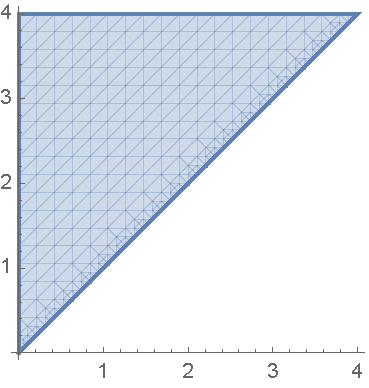
\includegraphics[width=.4\linewidth]{hw3_plot7a}
  \caption{Problem 7(a)}
  %\label{fig:test1}
\end{minipage}%
\begin{minipage}{.5\textwidth}
  \centering
  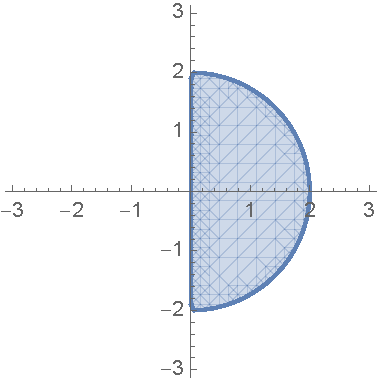
\includegraphics[width=.4\linewidth]{hw3_plot7b}
  \caption{Problem 7(b)}
 %\label{fig:test2}
\end{minipage}
\end{figure}

\begin{figure}[h]
\centering
\begin{minipage}{.5\textwidth}
  \centering
  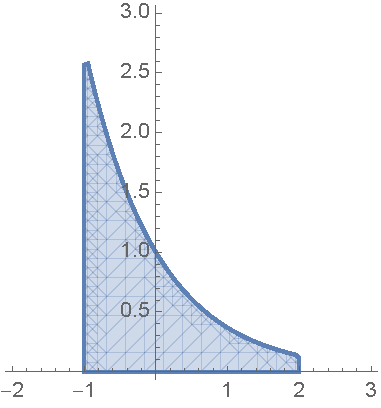
\includegraphics[width=.4\linewidth]{hw3_plot7c}
  \caption{Problem 7(c)}
  %\label{fig:test3}
\end{minipage}%
\begin{minipage}{.5\textwidth}
  \centering
  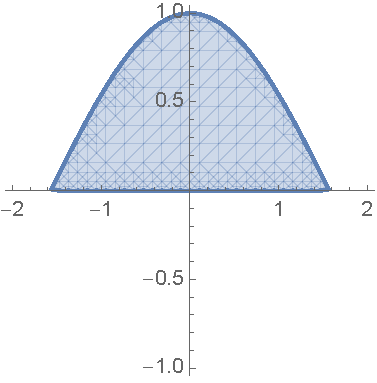
\includegraphics[width=.4\linewidth]{hw3_plot7d}
  \caption{Problem 7(d)}
 %\label{fig:test4}
\end{minipage}
\end{figure}

\end{newsolution}

\begin{exercise}{8}
Compute each of the iterated integrals below (note: you may need to switch the order of integration first). 
\begin{itemize}
\item[(a)] 
\begin{equation*}
\int_{1}^{4} \int_{1}^{\sqrt{x}} 2ye^{-x} dy dx
\end{equation*}
\item[(b)] 
\begin{equation*}
\int_{0}^{4} \int_{\sqrt{x}}^{2} \frac{3}{2+y^3}dy dx 
\end{equation*}
\item[(c)] 
\begin{equation*}
\int_{0}^{\frac{\pi}{2}} \int_{0}^{\sin(\theta)} \theta r dr d\theta
\end{equation*}
\item[(d)] 
\begin{equation*}
\int_{0}^{1} \int_{y}^{1} \sin(x^2) dx dy
\end{equation*}
\item[(e)] 
\begin{equation*}
\int_{1}^{\infty} \int_{0}^{\frac{1}{x}} y dy dx
\end{equation*}
\item[(f)] 
\begin{equation*}
\int_{0}^{\infty} \int_{0}^{\infty} xye^{-(x^2+y^2)} dx dy
\end{equation*}
\end{itemize}
\end{exercise}

\begin{newsolution}
The integrals which simplify in the opposite order of integration are indicated below. 
\begin{itemize}
\item[(b)] 
\begin{equation*}
\int_{0}^{4} \int_{\sqrt{x}}^{2} \frac{3}{2+y^3}dy dx  = \int_{0}^{2} \int_{0}^{y^2} \frac{3}{2+y^3} dx dy
\end{equation*}
\item[(d)] 
\begin{equation*}
\int_{0}^{1}\int_{y}^{1} \sin(x^2) dx dy = \int_{0}^{1} \int_{0}^{x} \sin(x^2) dy dx
\end{equation*}
\end{itemize}
\end{newsolution}

\begin{exercise}{9}
For each of the following problems, sketch the region of integration, set up the double integral for both orders of integration, and choose the most convenient order to evaluate the integrals.

\begin{itemize}
\item[(a)]
\begin{equation*}
\iint_{R} xy \ dA,
\end{equation*}
where $R$ is the rectangle with vertices $(0,0), (0,5), (3,5), (3,0)$. 
\item[(b)]
\begin{equation*}
\iint_{R} -2y\  dA,
\end{equation*}
where $R$ is the region bounded by $y=4-x^2$ and $y=4-x$. 
\item[(c)]
\begin{equation*}
\iint_{R} \frac{y}{1+x^2}\  dA,
\end{equation*}
where $R$ is the region bounded by $y=0, y=\sqrt{x}$ (for $x \geq 0$), and $x=4$. 
\item[(d)]
\begin{equation*}
\iint_{R} x^2+y^2 \ dA,
\end{equation*}
where $R$ is the semicircle bounded by $y=\sqrt{4-x^2}$, $y=0$. 
\end{itemize}
\end{exercise}

\begin{newsolution}
\begin{itemize}
\item[(a)] The integral can be expressed as
\begin{equation*}
\iint_{R} xy dA  = \int_{0}^{5} \int_{0}^{3} xy \ dx dy = \int_{0}^{3} \int_{0}^{5} xy \ dy dx. 
\end{equation*}
Both forms are simple enough to integrate directly. 
\item[(b)] The curves $y=4-x^2$ and $y=4-x$ intersect at $(0,4)$, $(1,3)$. The integral can be expressed as
\begin{equation*}
\iint_{R} -2y\  dA = \int_{0}^{1} \int_{4-x^2}^{4-x} -2y  \ dy dx = \int_{3}^{4} \int_{\sqrt{4-y}}^{4-y} -2y \ dx dy.
\end{equation*}
Both integrals can be easily evaluated. 
\item[(c)] The curves $y=0, y=\sqrt{x}$ (for $x \geq 0$) intersect at $(0,0)$, while the curves $y=\sqrt{x}, x=4$ intersect at $(4,2)$. Thus the integral can be written as 
\begin{equation*}
\iint_{R} \frac{y}{1+x^2}\  dA = \int_{0}^{4} \int_{0}^{\sqrt{x}}  \frac{y}{1+x^2} \ dy dx = \int_{0}^{2} \int_{y^2}^{4}  \frac{y}{1+x^2} \ dx dy.
\end{equation*}
The simpler integral is 
\begin{equation*}
\int_{0}^{4} \int_{0}^{\sqrt{x}}  \frac{y}{1+x^2} \ dy dx  = \int_{0}^{4} \frac{x}{2(1+x^2)} \ dx = \frac{\ln(17)}{4}.
\end{equation*}
\item[(d)] This integral can be written as 
\begin{equation*}
\iint_{R} x^2+y^2 \ dA = \int_{-2}^{2} \int_{0}^{\sqrt{4-x^2}} x^2+y^2 \ dy dx = \int_{0}^{2} \int_{-\sqrt{4-y^2}}^{\sqrt{4-y^2}} x^2+ y^2 \ dx dy.
\end{equation*}
The first iterated integral amounts to 
\begin{equation*}
\int_{-2}^{2} \int_{0}^{\sqrt{4-x^2}} x^2+y^2 \ dy dx = \int_{-2}^{2} \left[ x^2\sqrt{4-x^2} + \frac{(4-x^2)^{\frac{3}{2}}}{3}\right] dx = 4\pi
\end{equation*}
\end{itemize}
\end{newsolution}

\begin{exercise}{10}
Find the volume of the solid bounded by the relations. 
\begin{equation*}
z=\frac{1}{1+y^2}, x=0, x=2, y \geq 0.
\end{equation*}
\end{exercise}

\begin{newsolution}
The double integral you wish to evaluate is 
\begin{equation*}
\int_{0}^{2} \int_{0}^{\infty} \frac{1}{1+y^2} dy dx.
\end{equation*}
This integral is easily solved with the substitution $y = \tan(u)$. 
\end{newsolution}

\begin{exercise}{11}
Use polar coordinates to find the areas of the regions indicated below. 
\begin{parts}
\part The region inside the cardioid $r=2+\cos(\theta)$ and outside the circle $r=1$. 
\part The region inside the rose curve $r=4\sin(3\theta)$ and outside the circle $r=2$. 
\end{parts}
\end{exercise}

\begin{newsolution}
\begin{parts}
\part The integral one needs to compute is
\begin{equation*}
\int_{0}^{2\pi} \int_{1}^{2+\cos(\theta)} rdr d\theta
\end{equation*}
\part The rose curve has three petals, and the region inside the rose curve and outside the circle has three components, one in each petal, all of which are congruent (hence have the same area). We shall describe one of the integrals needed to compute the area (the result of which should be multiplied by three to obtain the total area of the region desired).  
\begin{equation*}
\int_{\frac{\pi}{18}}^{\frac{5\pi}{18}} \int_{2}^{4\sin(3\theta)} r dr d\theta.
\end{equation*}
\end{parts}
\end{newsolution}

\begin{exercise}{12}
Set up the triple integrals whose values describe the volumes of the solids indicated below. Do not compute the integrals. 
\begin{itemize}
\item[(a)] The solid bounded by $z=9-x^2$, $z=0$, $y=0$ and $y=2x$. 
\item[(b)] The solid bounded above by the paraboloid $z=4-x^2$ and below by the paraboloid $z=x^2+3y^2$. 
\end{itemize}
\end{exercise}

\begin{newsolution}
\begin{itemize}
\item[(a)] The solid region whose volume we wish to compute has two components: one for $x \leq 0$, one for $x\geq 0$. The minimum and maximum values of $x$ so that $9-x^2 \geq 0$ are $x_{\textrm{min}}=-3, x_{\textrm{max}}=3$. We will use $x$ as our free variable of integration. The volume can be computed  as 
\begin{equation*}
\int_{-3}^{0} \int_{2x}^{0} \int_{0}^{9-x^2} 1 dz dy dx + \int_{0}^{3} \int_{0}^{2x} \int_{0}^{9-x^2} 1 dz dy dx
\end{equation*}
\item[(b)] The surfaces $z=4-x^2$ and $z=x^2+3y^2$ intersect along a curve, whose projection onto the $xy$-axis is given by the equation 
\begin{equation*}
2x^2+3y^2 = 4.
\end{equation*}
This equation describes the an elipse in the $xy$-plane, and it will serve as the guide to set up a double integral in these two coordinates. The triple integral can be written as 
\begin{equation*}
\int_{-\sqrt{2}}^{\sqrt{2}} \int_{-\sqrt{\frac{4-2x^2}{3}}}^{\sqrt{\frac{4-2x^2}{3}}} \int_{x^2+3y^2}^{4-x^2} 1 dz dy dx 
\end{equation*}
\end{itemize}
\end{newsolution}

\begin{exercise}{13}
Convert the integrals below from rectangular to both spherical and cylindrical coordinates. Then evaluate the integral in one of its forms. 
\begin{itemize}
\item[(a)]
\begin{equation*}
\int_{0}^{2} \int_{0}^{\sqrt{4-x^2}} \int_{0}^{\sqrt{16-x^2-y^2}} \sqrt{x^2+y^2} dz dy dx
\end{equation*}
\item[(b)]
\begin{equation*}
\int_{-1}^{1} \int_{-\sqrt{1-x^2}}^{\sqrt{1-x^2}} \int_{1}^{1+\sqrt{1-x^2-y^2}} x dz dy dx
\end{equation*}
\end{itemize}
\end{exercise}

\begin{newsolution}
\begin{itemize}
\item[(a)] The integral can be written in cylindrical coordinates as 
\begin{equation*}
\int_{0}^{\frac{\pi}{2}} \int_{0}^{2} \int_{0}^{\sqrt{16-r^2}}  r^2\    dz dr d\theta
\end{equation*}
In spherical coordinates, the integral needs to be broken down into two:
\begin{equation*}
\int_{0}^{\frac{\pi}{2}} \int_{0}^{\frac{\pi}{6}} \int_{0}^{4} [\rho\sin(\theta)] \rho^2\sin(\phi) d\rho d\phi d \theta + \int_{0}^{\frac{\pi}{2}} \int_{\frac{\pi}{6}}^{\frac{\pi}{2}} \int_{0}^{\frac{2}{\sin(\phi)}} [\rho\sin(\theta)] \rho^2\sin(\phi) d\rho d\phi d\theta
\end{equation*}
\end{itemize}
\end{newsolution}

\begin{exercise}{14}
Find the Jacobians of the changes of variables indicated below. 
\begin{itemize}
\item[(a)] $x=-\frac{1}{2}(u-v)$, $y=\frac{1}{2}(u+v)$
\item[(b)] $x=e^u\sin(v)$, $y=e^u\cos(v)$. 
\item[(c)] $x=4u-v$, $y=4v-w$, $z=u+w$. 
\item[(d)] $x=r\cos(\theta)$, $y=r\sin(\theta)$.
\item[(e)]  $x=\rho \sin(\phi) \cos(\theta)$, $y=\rho \sin(\phi) \sin(\theta)$, $z=\rho \cos(\phi)$.
\item[(f)] $x=r\cos(\theta)$, $y=r\sin(\theta)$, $z=z$. 
\end{itemize}
\end{exercise}

\begin{exercise}{15} 
In each of the problems below, use a change of variables to compute the volumes of the regions indicated. 
\begin{itemize}
\item[(a)] The region below the graph of $f(x,y)=9xy$, and above the square with vertices $(1,0)$, $(0,1)$, $(1,2)$ and $(2,1)$ in the $xy$-plane. 
\item[(b)] The region bounded by the graph of $f(x,y)=(3x+2y)(2y-x)^{\frac{3}{2}}$ and the parallelogram $R$ with vertices $(0,0), (-2,3), (2,5)$ and $(4,2)$ in the $xy$-plane. 
\item[(c)] The solid bounded above by the graph of $f(x,y)=\frac{xy}{1+x^2y^2}$, and bounded below by the planar region bounded by the curves $xy=1$, $xy=4$, $x=1$ and $x=4$ in the $xy$-plane. 
\end{itemize}
\end{exercise}

\begin{newsolution}
\begin{itemize}
\item[(a)] Use the change of coordinates $u=y-x$ and $v=y+x$. Then the integral becomes
\begin{equation*}
\int_{-1}^{1} \int_{1}^{3} 9\left(\frac{u+v}{2}\right) \left(\frac{v-u}{2}\right) dv du =36.
\end{equation*}
\item[(c)] Use the change of variables $u=x, v=xy$, whose Jacobian determinant is $u$. In these coordinates, the integral becomes 
\begin{equation*}
\int_{1}^{4} \int_{1}^{4} \frac{v}{1+v^2} u\ dudv = \frac{15}{4}\ln\left(\frac{17}{2}\right).
\end{equation*}
\end{itemize}
\end{newsolution}
\end{document}